\documentclass[letterpaper, reqno,11pt]{article}
\usepackage[margin=1.0in]{geometry}
\usepackage{color,latexsym,amsmath,amssymb,graphicx, float}
\usepackage{hyperref}

\hypersetup{
colorlinks=true,
linkcolor=magenta,
filecolor=magenta,
urlcolor=cyan,
}

\graphicspath{ {images/} }

\begin{document}
\pagenumbering{arabic}
\title{PHYS 350 Final Project}
\date{April 11, 2022}
\author{Xander Naumenko, 38198354}
\maketitle

\tableofcontents

\section{Introduction}
 
The goal of this paper is to explore the consequences of alternate physical laws in Lagrangian mechanics, and how they affect the many results found throughout the course. [TBC]

\section{Gravitational Potential}

One fundamental law that yields surprisingly beautiful results is the fact that the gravitational potential goes with $\frac{1}{r}$. But it is interesting to explore how exactly physical systems evolve when this isn't the case. Here we will explore gravitational potentials of the form: 
\[
U(r)=-\frac{G_nm_1m_2}{r^{n}}=-\frac{\alpha}{r^{n}}
,\]
where $G_n$ is an arbitrary constant to make length scales more reasonable. Specifically we will focus on the case of the two body problem and the resultant orbits with these other reciprocal laws. In class we derived up to the expression for effective potential without making reference to the specific (radial dependent) gravitational potential. As this was derived in class the derivation will not be repeated, but for a system of two bodies of mass $ m_1, m_2$, position $\vec r_1, \vec r_2$ and initial conditions, we found that 
\[
\vec r_{cm}=\frac{m_1\vec r_1+m_2\vec r_2}{m_1+m_2}
,\]
\[
\vec r_{rel}=\vec r_2-\vec r_1
,\]
\[
\vec r_{cm}=\vec v_{cm, \text{initial}}t+\vec r_{cm, \text{initial}}
.\]
Thus the only part needed to solve is the relative motion. For convenience $r$ without subscript will be used to represent $|\vec r_{rel}|$. Then we also found that 
 \[
U_{eff}(r)=\frac{l^2}{2\mu r^2}+U(r)
\]
where $l=\left| r_0\times \mu\vec v_0 \right| $. The obvious next step is to find the equilibrium orbit distant, i.e. the point where $\frac{dU}{dr}=0$. Here we see the first interesting effect of our alternate potential: for any $n\neq 2$, solving for the equilibrium distance $p$ gives us
\[
\frac{dU}{dr}=-\frac{l^2}{\mu p^3}+\frac{n\alpha}{p^{n+1}}=0\implies p_n=\left( \frac{\mu}{l^2 n\alpha} \right)^{1 /(3-n-1)}
\]
which matches $p=\frac{l^2}{\mu\alpha}$ for $n=1$. However, if $n=2$ then this isn't valid since we're dividing by zero, so the $n=2$ case just reduces to
\[
U_{eff}=\left( \frac{l^2}{2\mu}-\alpha \right)\frac{1}{r^2}\equiv \frac{C}{r^2}
.\]
This is missing the characteristic well that the effective potential normally exhibits, which means that depending on the initial conditions, the relative distance will either got to infinity or $0$ depending on whether $C\geq 0$. To get an intuitive feel for how these different potentials behave, they are graphed in figure \ref{fig:U-plots}. 

\begin{figure}[htpb]
    \centering
    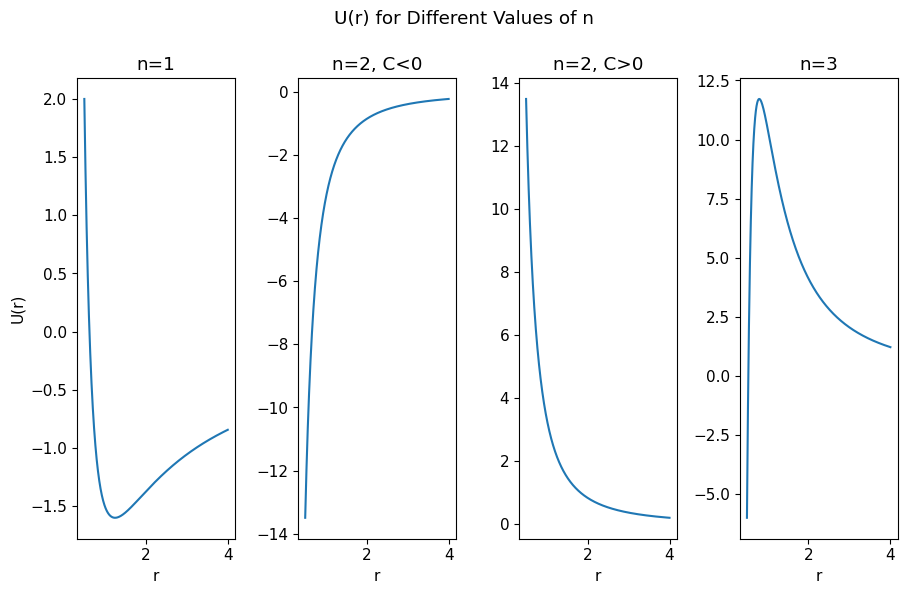
\includegraphics[width=0.8\textwidth]{U-plots}
    \caption{Plots of the shapes of potentials resulting from different values of n. The middle two are both the $n=2$ case, with the left one being with $C>0$ and the other with $C<0$. }
    \label{fig:U-plots}
\end{figure}

\end{document}
